\documentclass[a4paper,9pt]{jsarticle}
\usepackage{stdrep}

\title{宣言型プログラム論 ミニプロジェクト2}
\author{200911434 青木大祐}

\begin{document}
\maketitle
\newpage

\section{座標 (x,y) に,指定した色で半径 r の円に内接する正 n 角形を描画
 する関数}
\subsection{ソースコード}
\lstinputlisting{1.ml}

$range$関数はnからmまで1つずつ増加する数のリストを生成する関数である。こ
れを用いてそれぞれの頂点を{\it{fold\_left}}で処理している。

\subsection{実行例}
\begin{lstlisting}
# #use "1.ml";;
val range : int -> int -> int list = <fun>
val pi : float = 3.141592
val draw_regular_ngon :
  float -> float -> float -> Graphics.color -> int -> int = <fun>
File "1.ml", line 33, characters 2-29:
Warning 10: this expression should have type unit.
val main : float -> float -> float -> Graphics.color -> int -> unit = <fun>

# main 50.0 50.0 50.0 Graphics.green 10;;
\end{lstlisting}
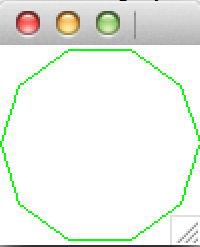
\includegraphics[width=5cm]{1_1.png} 



\section{座標 (x,y) に,指定された色で,与えられた図形を描画する}
\subsection{ソースコード}
\lstinputlisting{2.ml}

\subsection{実行例}
\subsubsection{三角形}
\begin{lstlisting}
# #use "2.ml";;
type figure =
    Rectangle of float * float
  | Circle of float
  | Triangle of float * float
val draw_figure : float -> float -> figure -> unit = <fun>
val main : float -> float -> Graphics.color -> figure -> unit = <fun>

# main 10.0 10.0 red (Triangle(30.0,40.0));;
\end{lstlisting}

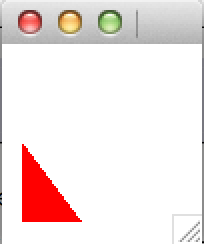
\includegraphics[width=5cm]{2_1.png}
\newpage
\subsubsection{円}
\begin{lstlisting}
# main 50.0 50.0 red (Circle(30.0));;
\end{lstlisting}

\includegraphics[width=5cm]{2_2.png}

\subsubsection{四角形}
\begin{lstlisting}
# main 10.0 10.0 red (Rectangle(20.0, 40.0));;
\end{lstlisting}

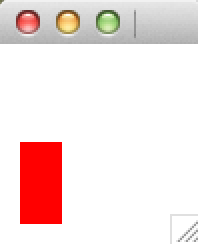
\includegraphics[width=5cm]{2_3.png}

\newpage
\section{図形を組み合わせた図形}
\subsection{ソースコード}

\lstinputlisting{3.ml}

\subsection{実行例}
\subsubsection{例1}
\begin{lstlisting}
 # #use "3.ml";;
type figure =
    Rectangle of float * float
  | Circle of float
  | Triangle of float * float
val draw_figure : float -> float -> float -> figure -> unit = <fun>
type region =
    Figure of figure
  | Translate of float * float * region
  | Scale of float * region
  | Union of region * region
type picture = (Graphics.color * region) list
val draw_region : float -> float -> float -> region -> unit = <fun>
val draw_picture : (Graphics.color * region) list -> unit = <fun>
val ex : (Graphics.color * region) list =
  [(0,
    Union (Translate (25., 60., Figure (Circle 25.)),
     Translate (75., 60., Figure (Circle 25.))));
   (16711680, Translate (25., 0., Figure (Rectangle (50., 50.))))]
val main : (Graphics.color * region) list -> unit = <fun>
# main ex;;
\end{lstlisting}

\includegraphics[width=5cm]{3_1.png}

\subsubsection{例2}

\begin{lstlisting}                                                                                                                                    
let mypict =                                                                                                                                  
  let circle = Figure (Circle 25.) in                                                                                                         
  let r1 = Union (Translate (25.,60. ,Scale(1.25, circle)),                                                                                   
            Translate (75.,60. ,Scale(0.75, circle))) in                                                                                      
  let rectangle = Figure (Rectangle (50., 50.)) in                                                                                            
  let triangle = Figure (Triangle(35., 35.)) in                                                                                               
  let r2 = Union(Translate( 25., 0., rectangle),                                                                                              
                 Translate( 75., 75., Scale(0.25, triangle))) in                                                                              
  [(Graphics.green, r1); (Graphics.blue, r2)]                                                                                                 
;;                                                                                                                                            
\end{lstlisting}

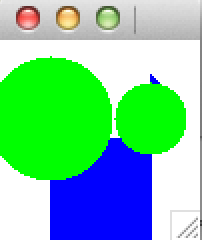
\includegraphics[width=5cm]{3_2.png}
\end{document}
